%%
%% This is file `mcmthesis-demo.tex',
%% generated with the docstrip utility.
%%
%% The original source files were:
%%
%% mcmthesis.dtx  (with options: `demo')
%% !Mode:: "TeX:UTF-8"
%% -----------------------------------
%% This is a generated file.
%% 
%% Copyright (C) 2010 -- 2015 by latexstudio
%%       2014 -- 2019 by Liam Huang
%%       2019 -- present by latexstudio.net
%% 
%% License: The LaTeX Project Public License 1.3c
%% 
%% The Current Maintainer of this work is latexstudio.net.
%% 
\documentclass{mcmthesis}
 %\documentclass[CTeX = true]{mcmthesis}  % 当使用 CTeX 套装时请注释上一行使用该行的设置
\mcmsetup{tstyle=\color{red}\bfseries,%修改题号,队号的颜色和加粗显示,黑色可以修改为 black
        tcn = 2412631, problem = C, %修改队号,参赛题号
        sheet = true, titleinsheet = true, keywordsinsheet = true,
        titlepage = false, abstract = false}

  %四款字体可以选择
  %\usepackage{times}
  \usepackage{newtxtext,newtxmath} %CTeX 无此字体,可用 txfonts 替代,请使用新版 TeXLive.
  %\usepackage{palatino}
  %\usepackage{txfonts}

\usepackage{indentfirst}  %首行缩进,注释掉,首行就不再缩进。
\usepackage{lipsum}
\title{Momentum in Tennis}
\begin{document}
\begin{abstract}
\par What's the "momentum" in tennis? A classic game is the 2023 Wimbledon Gentlemen’s final where Carlos Alcaraz defeated Novak Djokovic. This match highlighted significant shifts in momentum, challenging the traditional understanding and measurement of this phenomenon in sports. Despite leading or trailing, players exhibited remarkable comebacks, attributed to momentum shifts. However, what is momentum? What are the factors that affect momentum? In this paper, we will delve into the influence of momentum in a game.

Firstly, we construct a \textbf{performance model} that macroscopically characterizes a player's performance state in a game based on the impact of serving on scoring. The output of this model is the $\bigtriangleup performance$ score obtained by the contestant at a certain moment. The performance score of the contestant at a certain moment is obtained by adding up all $\bigtriangleup performance$ scores before that moment. When a match ends, the player with a higher performance score should win the match. We apply the performance model to 31 matches in the dataset, and in the end, only 3 predicted results are incorrect, with an accuracy rate of 90.323\%. 

Secondly, we conduct a series of independent tests on the factors that may affect the direction of the match. We first conduct \textbf{Chi-Square} tests and \textbf{Pearson coefficient} tests on the output results of the performance model to verify the correlation between variables and scores. Finally, we calculate the distribution of consecutive scores of players in the match and verify that this distribution is not a normal or geometric distribution, thereby proving that consecutive scores of players in the competition are not random events.

Thirdly, we select 16 factors that may affect the score, and through binary logistic regression analysis and covariance matrix construction, we filter out 16 factors to 8 factors. We used five models, namely LGBM, XGB, SVC, MLP, and LR, to learn based on these 8 factors and actual scores. We hope that the model can predict the real-time score situation in a game well. In the end, the MLP model stands out with an Accuracy of 73.8\% and a Precision of 75.4\%. Next, we aggregate the data from the point dimension of a game to the game dimension, enabling MLP to ultimately predict the score of a game.

Fourthly, we define the "trend change" in a match - which is also the most direct explanation of momentum. We use the MLP model to predict the game score results and find the change in the score difference between two players in a match. We use \textbf{KMeans} clustering to find the turning point in a match. Next, we annotate these points in a match and redesign a \textbf{support vector machine model} to predict game turning points based on the 8 factors mentioned earlier.

Finally, we validate the generalization ability of the constructed support vector machine model. We select data from another final of Djokovic in 2016, and the final output of the model reflect the changes in the score of the game. However, in the data of another women's singles match, the model's predictions are not accurate enough, which also prompts us to think about other factors.
\begin{keywords}
\textbf{Momentum; Tennis; Pearson coefficient; KMeans; Support Vector Machine}
\end{keywords}
\end{abstract}
\maketitle
%% Generate the Table of Contents, if it's needed.
\tableofcontents
\newpage
%%
%% Generate the Memorandum, if it's needed.
%% \memoto{\LaTeX{}studio}
%% \memofrom{Liam Huang}
%% \memosubject{Happy \TeX{}ing!}
%% \memodate{\today}
%% \memologo{\LARGE I'm pretending to be a LOGO!}
%% \begin{memo}[Memorandum]
%%   \lipsum[1-3]
%% \end{memo}
%%
\section{Introduction}
\subsection{Background}
Tennis is a competitive sport with a long history. Many factors affect the trend of the game. In the 2023 Wimbledon Gentlemen's final, Djokovic dominated the first set 6 - 1, which convinced everyone that he seemed destined to win easily. However, the second set wasn't as easy as the first. Eventually Alcarez won in a tie-breaker 7-6. The third set where Alcaraz won handily 6 - 1 was totally the reverse of the first. Alcarez seemed to dominate the match and win the champion. However, in the fourth set, Djokovic took complete control to win 6 - 3. Everyone all thought that Djokovic had the advantage from the fourth set, but again a change of direction occurred and Alcaraz gained control and finally won 6 - 4. What happened in this match? One common explanation is that the momentum plays a major role. However, what factors affect momentum and how to measure the momentum are ambiguous. So in this paper we focus on this problem.
\subsection{Restatement of the Problem}
Data provided is a file of every point from all Wimbledon 2023 men’s matches after the first 2 rounds. The file includes the number of the match, the names of the players, the elapsed time, the number of the point, game and set, the sets the players have won, the score, the server, the victor, the ace, the shot type and the running distance of the players.

We need to develop models to determine and solve the following problems:
\begin{itemize}
  \item \textbf{Problem 1:} Develop a model to capture the flow of play as points occur. The model should identify which player is performing better at a given time in the match. What's more, the model should measure how much better they are performing.
  \item \textbf{Problem 2:} Is the fluctuation and consecutive scores of players in a game a random event? We need to verify the correlation through some testing methods.
  \item \textbf{Problem 3:} Explore some relevant factors that affect the trend of the match, establish a model that can predict fluctuations in the match, and explore the ones that have the greatest impact on matches fluctuations among these factors. Then, based on these factors, provide match recommendations for one tennis player.
  \item \textbf{Problem 4:} Test the model's generalization ability on other competition data and consider potential factors that may need to be considered.
\end{itemize}


\section{Preparation for modeling}
\subsection{Model Assumptions}
We have made the following model assumptions regarding this issue:
\begin{enumerate}
  \item Assuming that the provided tennis match data is sufficient to reflect the actual situation on the field.
  \item Assuming that a player's skill level is fixed during the game and not affected by factors such as injury, psychological pressure, etc.
  \item Assuming that natural factors such as wind direction and lighting have no impact on the competition.
  \item Assuming there are no negative external factors such as gambling that may alter the outcome of the competition.
\end{enumerate}

\subsection{Notations}
Table 1 provides a unified explanation of the symbols used in the formulas presented in this article.
\begin{table}[]
	\centering
	\begin{tabular}{cl}
		\hline
		\textbf{Symbol}   & \textbf{Description}                                                                     \\ \hline
		$S_{1i}$ & The score of the first player in the i-th game                                  \\ \hline
		$S_{2i}$ & The score of the second player in the i-th game                                 \\ \hline
		$P_i$    & The difference in scores between the two players in the i-th game               \\ \hline
		$TP_i$   & The difference in scores between adjacent games                                 \\ \hline
		$p_{1i}$ & The probability of the first player getting the i-th point                      \\ \hline
		$p_{2i}$ & The probability of the second contestant getting the i-th point                 \\ \hline
		$prob_i$ & The difference in scoring probability between the two players on the i-th point \\ \hline
		$dp_i$   & The difference in the probability difference of scoring within a step size      \\ \hline
	\end{tabular}
	\caption{Notations}
	\label{tab:my-table}
\end{table}

\subsection{Dataset}
The dataset contains relevant data on Wimbledon tennis matches, covering 7284 data points, including 46 fields, including game ID, player name, game time, game sets, innings, scores, as well as data on player scores, serve, winning points, double errors, non forced errors, running distance, serving speed, and other aspects.

We have conducted statistics on some of the interesting data:
\begin{itemize}
  \item The dataset contains a total of 31 games.
  \item Player1 and Player2 each contain 19 and 22 players, with Carlos Alcaraz and Novak Djokovic appearing the most frequently, making them the final finalists.
  \item The average serving speed is about 112 miles per hour, ranging from 72 to 141 miles per hour, indicating a wide distribution of serving strength.
\end{itemize}

Since we do not initially use all the indicators provided in the dataset, we only perform a simple outlier removal task. The detailed data processing process is presented in Section 5.2.




\section{Quantify the Performance of the Players}
\subsection{Feature Choosing}
For Task 1, We first conduct some preliminary explorations.
We begin the first task of exploring factors that can measure a player's performance in a competition. In terms of objective factors, in tennis match, players who usually serve have a higher probability of scoring. In terms of subjective factors, the change in morale during the competition is a decisive factor in the mentality of players, which to some extent affects their performance. So in terms of objective factors, we choose serving scores and breaking as factors, and in terms of subjective factors, we choose winning streak as factors.
\subsection{Model Building}
We select whether it is a serve round, whether the player breaks the serve and the length of the winning streak to model this task. We use a performance model to quantify the performance of players. Due to the advantage of the serving side in scoring, it can be considered that when a player scores in the opponent's serving round, he has better performance and can therefore earn more points. When a player scores in his serve round, he should receive slightly less points than the former. When a player breaks a serve in the serving round, we believe it will have an impact on his mentality, thereby affecting his performance score to a certain extent. Meanwhile, we believe that when a player wins in a row, their momentum will be stronger, so we allow them to earn more extra points. Through this method, we quantify the performance of players in a game and present the changes in the performance in a game by accumulating their scores. In addition, we have defined a certain range of parameters for the model and conducted sufficient validation within this range, ultimately determining the optimal parameters. We also validated the effectiveness of the model using other competition data included in the dataset. 
\subsubsection{Model Abstraction}
The core formula of the performance model is defined as follows:
\[
	\bigtriangleup Performance = [ Base + ((\frac{e}{2})^{con - 1} - 1) \times bonus](1 \pm \alpha)(1 + \beta)
\]
In this formula, $Base$ represents the player's basic performance score, $\alpha$ represents the weight of the additional score obtained during the serve round score, and $\beta$ represents the weight of the additional score obtained after breaking serve. If there is no breaking serve, $\beta$ is 0. $con$ is the maximum length of the winning streak from this moment forward, and bonus is the additional performance score weight obtained from the winning streak. Through this formula, we can obtain the $\bigtriangleup performance$ at any moment. By adding up all $\bigtriangleup performance$ before this moment, we can characterize the performance score of the player at that moment. After a game is over, the absolute difference in performance score between the two players is the degree to which the winner performs better.

\subsubsection{Parameter Adjustment}
Normally, it is evident that at the end of a game, the winner of the match should have a higher performance score. In the above formula, $bonus$, $\alpha$, and $\beta$ are the parameters that need to be adjusted. We need to adjust the values of these three parameters to ensure that the player with higher performance score is the winner of the game.

We use a grid search parameter tuning method. In this task, we define accuracy as follows: 

Calculate the results of the model on all game data. If the winner in a certain game matches a player with a higher performance score output by the model, we believe that the model's prediction is correct. The accuracy is the number of matches correctly predicted by the model divided by the total number of matches.

During this process, the code traversed all combinations of three parameters $\alpha$, $\beta$, and $bonus$ to find the best performing parameter combination for the model. Specifically, for each pair of parameter combinations, it calculates the model's results on all competition data and selects the parameter with the highest accuracy as the optimal parameter.

In our experiment, the value space for $\alpha$ and $\beta$ is [0.01, 0.02, 0.03, 0.04, 0.05, 0.1], while the value space for $bonus$ is [0.01, 0.05, 0.1, 0.2, 0.5]. Through grid search, we found the optimal parameter combination ($\alpha$, $\beta$, $bonus$) as (0.05, 0.05, 0.01). Under this parameter combination, the accuracy of the model reached 90.32\%. We have plotted this result into a scatter plot, where the black boxed scatter points represent the matches with incorrect predictions, as shown in Figure 1. In addition, we also calculated the accuracy of the set and compared the results with the accuracy of the game, as shown in Figure 2.

\begin{figure}[h]
\centering
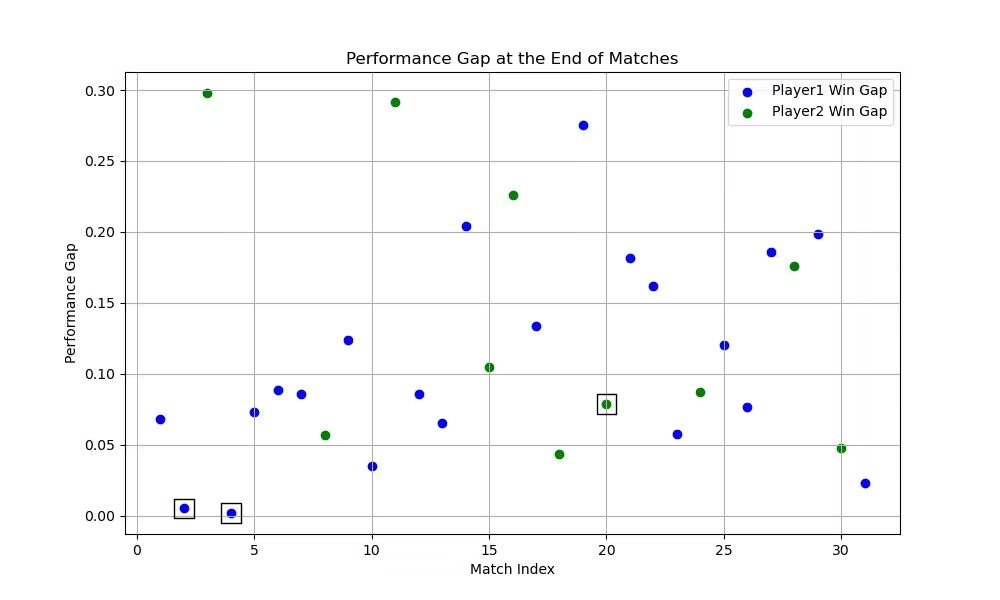
\includegraphics[width=12cm]{figures/Accuracy scatter plot.jpg}
\caption{The Accuracy Scatter Plot} \label{fig:aa}
\end{figure}

\begin{figure}[h]
\centering
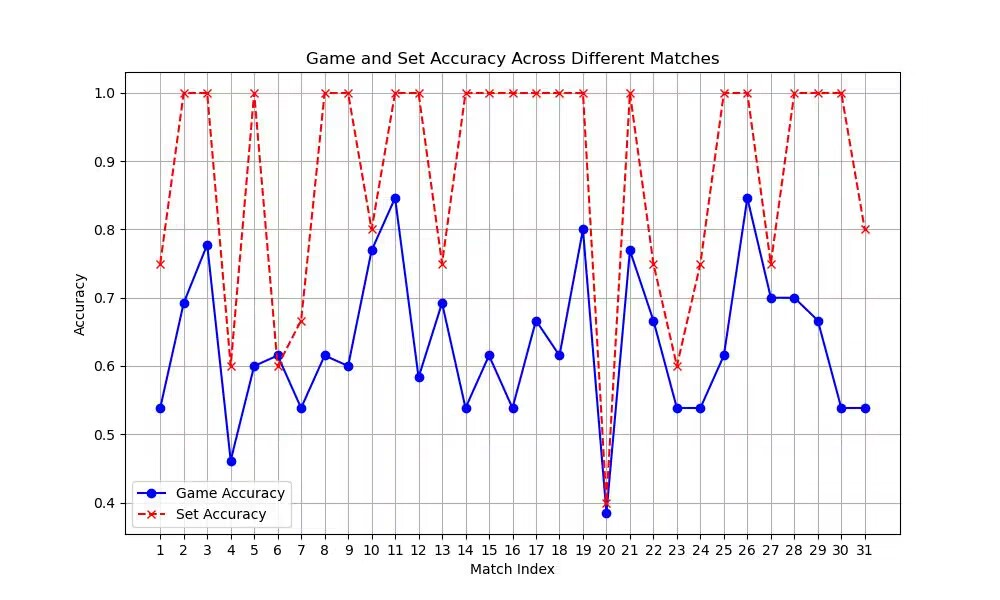
\includegraphics[width=12cm]{figures/set and game acc.jpg}
\caption{The Accuracy of Set and Game} \label{fig:aa}
\end{figure}

\subsubsection{Visual Analysis of Match Situation}
We mainly study the classic match between Djokovic and  Alcarez, with a total score of 3:2. We visualize and analyze the process of this match, and the performance score curves of the two players basically met the expected situation. 

At the same time, we also studied other matches included in the dataset and selected matches with a total score of 3:1 and a total score of 3:0 to draw visualization curves. The visualization results are shown in Figures 3, 4, and 5. The dotted line represents the end of the game, and the solid line represents the end of the set. Figure 3 corresponds to the classic game in the background of the problem. In the match corresponding to Figure 4, the first player wins one game and then loses one game before chasing two consecutive games, which is consistent with the curve situation in Figure 4: the blue line is above the orange line at the beginning, then slightly drops below the orange line for a period of time, and then rises again above the orange line until the game ends. In the match corresponding to Figure 5, the first player loses with a score of 0-3, as reflected in the figure: the blue line is above the orange line for a short period of time, but quickly falls below it and remains there until the end of the game.

\begin{figure}[h]
\centering
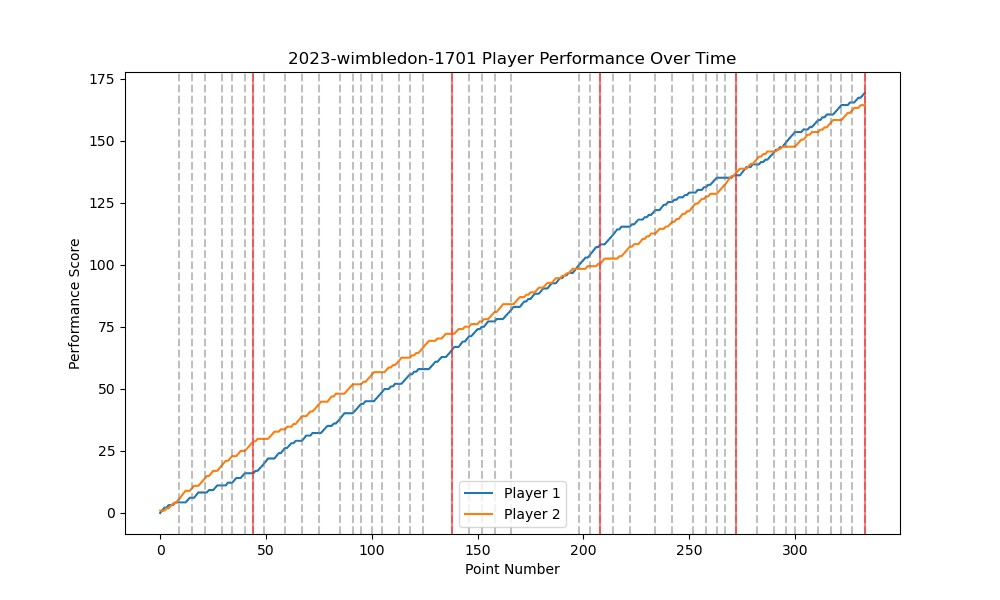
\includegraphics[width=12cm]{figures/32.JPG}
\caption{Match 3:2} \label{fig:aa}
\end{figure}

\begin{figure}[h]
\centering
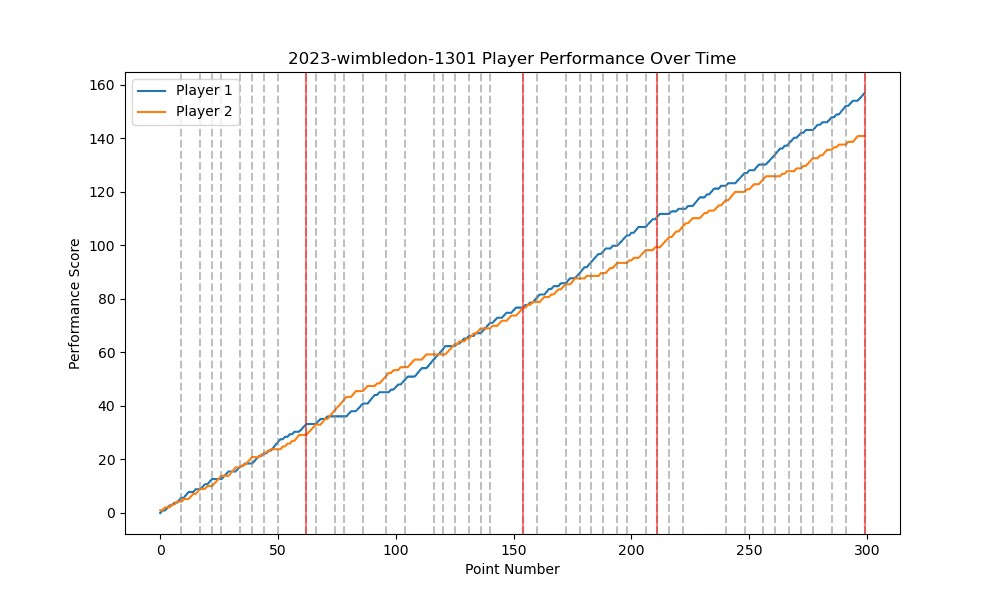
\includegraphics[width=12cm]{figures/31.JPG}
\caption{Match 3:1} \label{fig:aa}
\end{figure}

\begin{figure}[h]
\centering
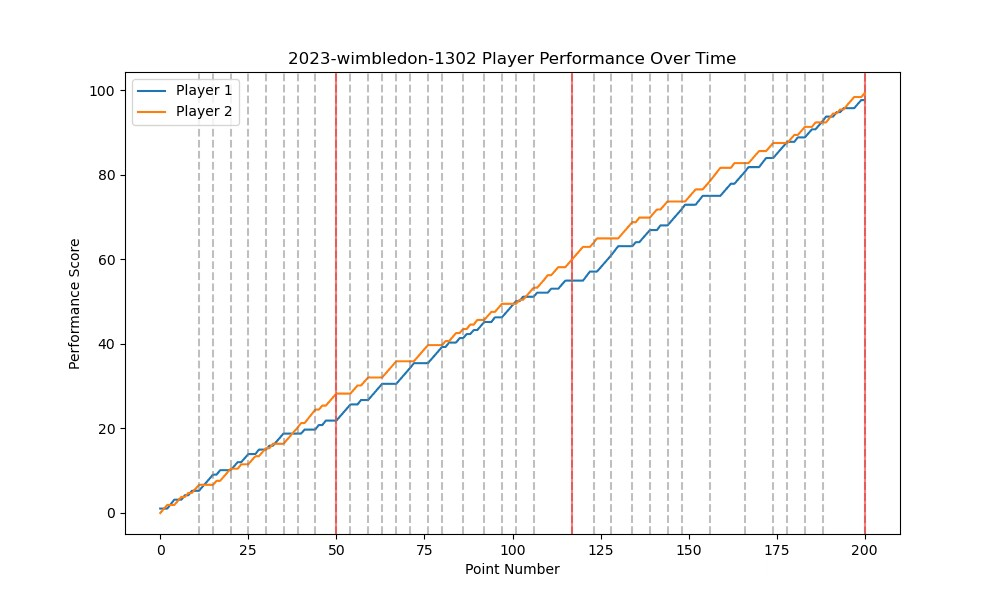
\includegraphics[width=12cm]{30}
\caption{Match 3:0} \label{fig:aa}
\end{figure}


\section{Does momentum play a role in a match?}
\subsection{Overall}
For Task 2, a tennis coach has a skeptical attitude towards the role of momentum in the game. He believes that the fluctuations in a game's situation and the continuous success of a player are both random occurrences, which goes against our intuition. So far, we have not conducted in-depth research on momentum. Momentum refers to the changes in a player's state during the match, so the performance score and real-time score proposed in the third and fourth sections can to some extent represent the concept of momentum. To verify whether momentum is useful in competitions, we will use three methods to verify this issue:
\begin{enumerate}
  \item We conduct a Chi-Square test on the results of the performance model introduced in section 3.2 to verify the correlation between performance scores and match results.
  \item We conduct a Pearson correlation coefficient test on the real-time performance score and actual score of the performance model in section 3.2 to verify the relationship between real-time performance score and actual score.
  \item We have calculated the distribution of consecutive scores of players in 31 matches to test whether their consecutive scores are random events.
\end{enumerate}
\subsection{The correlation between performance scores and match results}
\subsubsection{Chi-Square Test}
Chi Square Test is a commonly used hypothesis testing method in statistics, mainly used to test the independence between two categorical variables. The core idea is to compare whether the difference between the observed frequency and the expected frequency is significant. When conducting chi square tests, a cross tabulation should be created based on the classification of each categorical variable. The calculation formula for the chi square statistic is as follows:
\[
	\chi^{2}=\sum \frac{\left(O_{i j}-E_{i j}\right)^{2}}{E_{i j}}
\]
Among them, $O_{i j}$ represents the observation frequency in the i-th row and j-th column, $E_{i j}$ represents the expected frequency in the i-th row and j-th column, and the calculation formula for the expected frequency is:
\[
	E_{i j}=\frac{\left(O_{i} \times O_{j}\right)}{n}
\]
Among them, $O_i$ and $O_j$ represent the sum of observation frequencies in row i and column j, respectively, and n represents the total sample size.

\subsubsection{Result Validation}
We conduct a Chi-Square test on the performance scores and final competition results of the contestants in section 3.2 to verify whether their performance scores are related to the match results. We analyzed the results of 31 matches and the performance scores of the two players from the perspective of the first player in each match. We write the results in the form required for the chi square test, as shown in Table 2. The chi square test results show that the chi square statistic is 15.81, the degree of freedom is 1, and the P-value is 7.0025e-05, which is less than 0.05. Therefore, the null hypothesis can be rejected, that is, there is a significant difference between the two scenarios (p1>p2 and p2>p1) and the outcome.
\begin{table}[]
	\centering
	\begin{tabular}{cccc}
		\hline
		\textbf{Performance Scores} & \textbf{$P_1$ Win} & \textbf{$P_1$ Lose} & \textbf{Total} \\ \hline
		$P_1$ > $P_2$      & 19        & 2          & 21    \\ \hline
		$P_1$ < $P_2$      & 1         & 9          & 10    \\ \hline
		Total              & 20        & 11         & 31    \\ \hline
	\end{tabular}
	\caption{Score situation and distribution table of match results}
	\label{tab:my-table}
\end{table}

We propose the assumption $\mathcal{H}_0$: the performance score of the player and the result of the competition are independent.

\subsection{The correlation between predicted scores and actual scores}
\subsubsection{Pearson Correlation}
The Pearson correlation coefficient is a statistical measure that measures the degree of linear correlation between two variables. It describes the strength and direction of the linear relationship between two variables X and Y. Its value is between -1 and 1, and the closer the specific value is to 1 or -1, the stronger the linear correlation between the two variables; If the value is close to 0, it indicates that there is almost no linear correlation between the two variables.

The calculation formula for Pearson correlation coefficient is as follows:\[
	r_{x y}=\frac{\sum\left(x_{i}-\bar{x}\right)\left(y_{i}-\bar{y}\right)}{\sqrt{\sum\left(x_{i}-\bar{x}\right)^{2} \sum\left(y_{i}-\bar{y}\right)^{2}}}
\]
Here, $r_{x y}$ is the correlation coefficient between X and Y, $x_i$ and $y_i$ are the i-th observed values in X and Y, respectively, and $\bar{x}$ and $\bar{y}$ are the mean values of X and Y.

\subsubsection{Result Validation}
We have statistically analyzed the real-time performance score and actual score results output by the performance model in Section 3.2, and calculated the average real-time performance score and actual score. We propose the assumption $\mathcal{H}_0$: There is no correlation between real-time performance score and actual score. Then, we calculate the Pearson coefficient and the results are shown in Table 3. Therefore, we reject the null hypothesis.
\begin{table}[]
	\centering
	\begin{tabular}{ll}
		\hline
		\textbf{Metric}  & \textbf{Value} \\ \hline
		Pearson & 0.366 \\ \hline
		P-Value & 0.000 \\ \hline
	\end{tabular}
	\caption{the Pearson Coefficient}
	\label{tab:my-table}
\end{table}

\subsection{The probability Distribution of Consecutive Scores}
\subsubsection{Normal Distribution}
A normal distribution is a continuous probability distribution with a symmetrical bell shaped curve. Normal distribution is one of the most common probability distributions, which is very common in nature, social sciences, and many other fields. The characteristic of a normal distribution is that it has a unique peak and the distribution is symmetrical on both sides.

The basic formula for a normal distribution is as follows:\[
	f\left(x ; \mu, \sigma^{2}\right)=\frac{1}{\sigma \sqrt{2 \pi}} e^{-\frac{(x-\mu)^{2}}{2 \sigma^{2}}}
\]

In tennis, if the scoring situation is a random event and the probability of each ball being hit back is equal, then in a large number of matches, the frequency of consecutive scoring may approach a normal distribution.

\subsubsection{Geometric Distribution}
Geometric distribution is a discrete probability distribution that describes the location where the first successful event occurred in n independent Bernoulli experiments. The Bernoulli test refers to an experiment where there are only two possible outcomes, commonly referred to as "success" and "failure," and the probability of each outcome occurring is constant.

The basic formula for geometric distribution is as follows:
\[
	P(X=k)=(1-p)^{k-1} p
\]
In tennis, each return shot can be a successful or unsuccessful score, and can therefore be considered a Bernoulli test. If the probability of a successful score on each stroke is constant, the distribution of consecutive scores may follow a geometric distribution.

\subsubsection{Result Validation}
We counte the consecutive scoring situations in 31 matches, and the results are summarized in Table 4.
\begin{table}[]
	\centering
	\begin{tabular}{cc}
		\hline
		\textbf{consecutive score length} & \textbf{Frequency} \\ \hline
		2                       & 1000      \\ \hline
		3                       & 507       \\ \hline
		4                       & 447       \\ \hline
		5                       & 11        \\ \hline
		6                       & 1         \\ \hline
	\end{tabular}
	\caption{Summary of Consecutive Scores}
	\label{tab:my-table}
\end{table}

Draw a graph of the distribution of consecutive scores, as shown in Figure 9, and it is found that it cannot fit a normal distribution or a geometric distribution, indicating that consecutive scores are not a random event.

\begin{figure}[h]
\centering
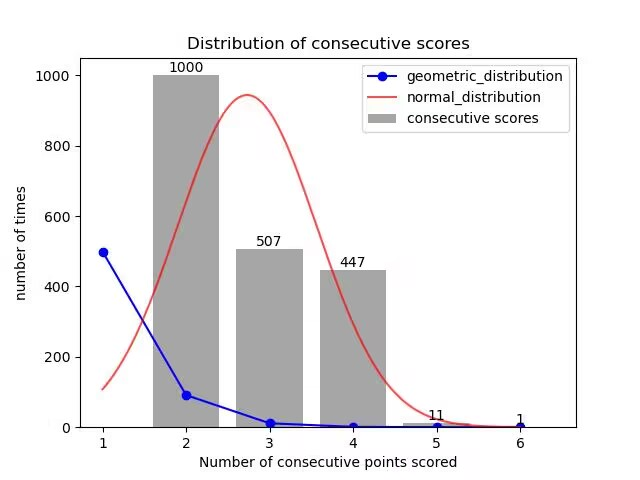
\includegraphics[width=12cm]{figures/Distribution.jpg}
\caption{Distribution of Consecutive Scores} \label{fig:aa}
\end{figure}


\section{Quantify player performance with machine learning models}
\subsection{Overview}
In Task 1, although the above performance model has been used to calculate the performance score of the contestant to quantify their performance, this method has shortcomings. In fact, the points received by players in a game are actually the most intuitive factor in their reaction state, but in the performance model above, points are ignored. Moreover, in the performance model above, since the performance score is only the accumulation of past scores, the player's past state has a significant impact on the final performance score. So we have relisted the factors that may affect player performance, explored the correlation between these factors and points from a micro perspective through binary logistic regression. Then we calculate the covariance matrix of these factors for further feature selection, and finally use five different machine learning models for modeling. By comparing the performance of these different machine learning models, we ultimately believe that the MLP model is capable of handling this task.

\subsection{Feature Selection}
The scoring situation is the most direct reflection of a player's state in a game. In addition to being the server, a player's point is also closely related to their personal technical and tactical level, physical exertion, and game mentality:
\begin{itemize}
  \item From the perspective of player skills and tactics, there are factors such as past and real-time player scores.
  \item From the perspective of player's physical exertion, the real-time total running distance of the athlete is taken as a factor.
  \item From the perspective of the player's competitive mentality, factors such as whether there are service errors, whether they win without extra time, and whether they score while the opponent was serving are considered.
\end{itemize}
Based on the above analysis, we have preliminarily selected 16 factors that affect real-time scores of players, as shown in Table 1:
% Please add the following required packages to your document preamble:
% \usepackage{longtable}
\begin{longtable}[c]{ll}
	\hline
	\textbf{Factor}                                                                                                 & \textbf{Sign} \\ \hline
	\endfirsthead
	\endhead
	The number of games won in the current set                                                             & $X_1$   \\ \hline
	The progress of leading the score in this game                                                         & $X_2$   \\ \hline
	Is it the server                                                                                       & $X_3$   \\ \hline
	Did the previous point score                                                                           & $X_4$   \\ \hline
	The progress of leading the score in this match                                                        & $X_5$   \\ \hline
	Is it a serve score                                                                                    & $X_6$   \\ \hline
	Whether to score a counterattack                                                                       & $X_7$   \\ \hline
	Forehand and Backhand in Scoring                                                                       & $X_8$   \\ \hline
	Are there any mistakes in this game                                                                    & $X_9$   \\ \hline
	Has there been any non coercive error in this game                                                     & $X_{10}$  \\ \hline
	The ratio of the number of times a player approaches the net to the score of their approach to the net & $X_{11}$  \\ \hline
	The ratio of the opponent's chances of scoring while serving to the actual score obtained              & $X_{12}$  \\ \hline
	The total distance run in this match                                                                   & $X_{13}$  \\ \hline
	The total distance run within the last three points                                                    & $X_{14}$  \\ \hline
	Previous point run distance                                                                            & $X_{15}$  \\ \hline
	Real time serving pace                                                                                 & $X_{16}$  \\ \hline
	\caption{Factors that affect real-time scores of players}
	\label{tab:my-table}
\end{longtable}
We removed samples with abnormal scores and some samples with missing pacing. Then, we standardized all the extracted features: We find the maximum and minimum values for each feature in the dataset, and then scale all features according to the following formula, so that the data range is scaled to between 0 and 1:
\[
	X_{\text {scaled }}=\frac{X-X_{\min }}{X_{\max }-X_{\min }}
\]

We conducted binary logistic regression analysis on the standardized data to determine the significance between these factors and scores. In the end, we excluded $X_4$, $X_{13}$, and $X_{14}$ because their significance remained at 0 even after retaining three decimal places. We further processed the remaining 13 variables and plotted their covariance matrix heatmaps, as shown in Figure 6.

\begin{figure}[h]
\centering
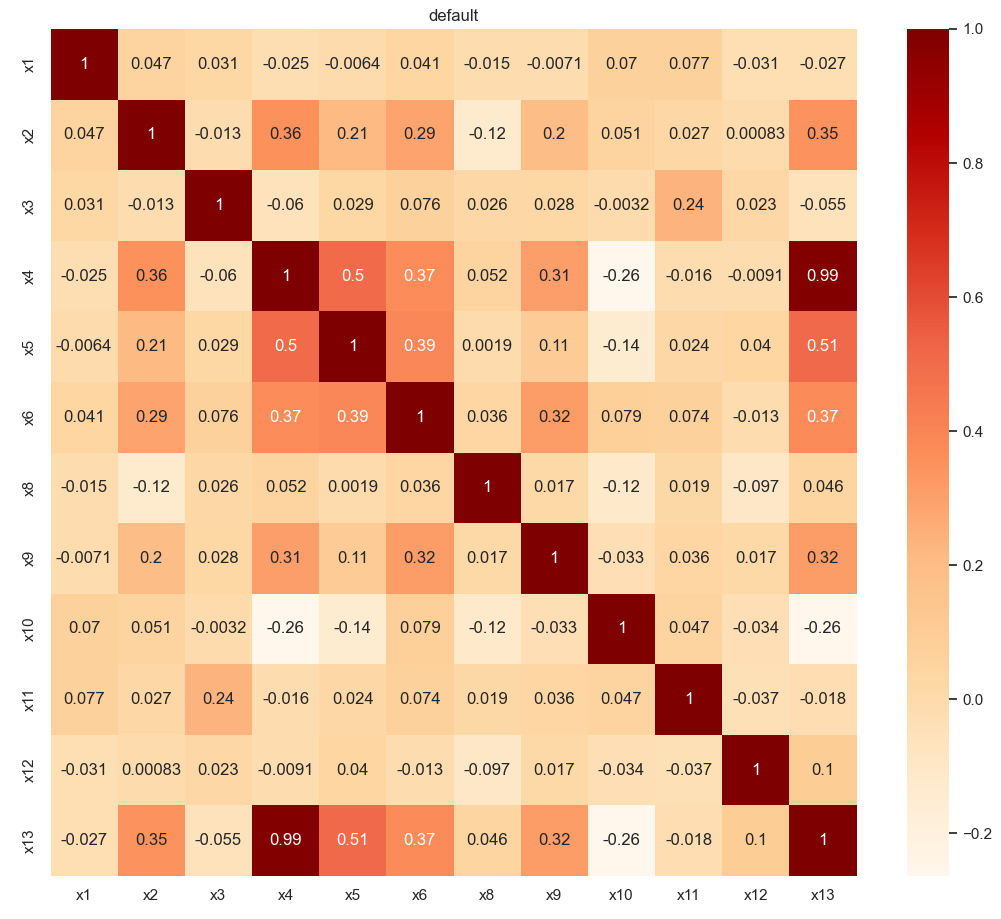
\includegraphics[width=12cm]{figures/covariance_matrix.png}
\caption{Covariance Matrix} \label{fig:aa}
\end{figure}

\begin{figure}[h]
\centering
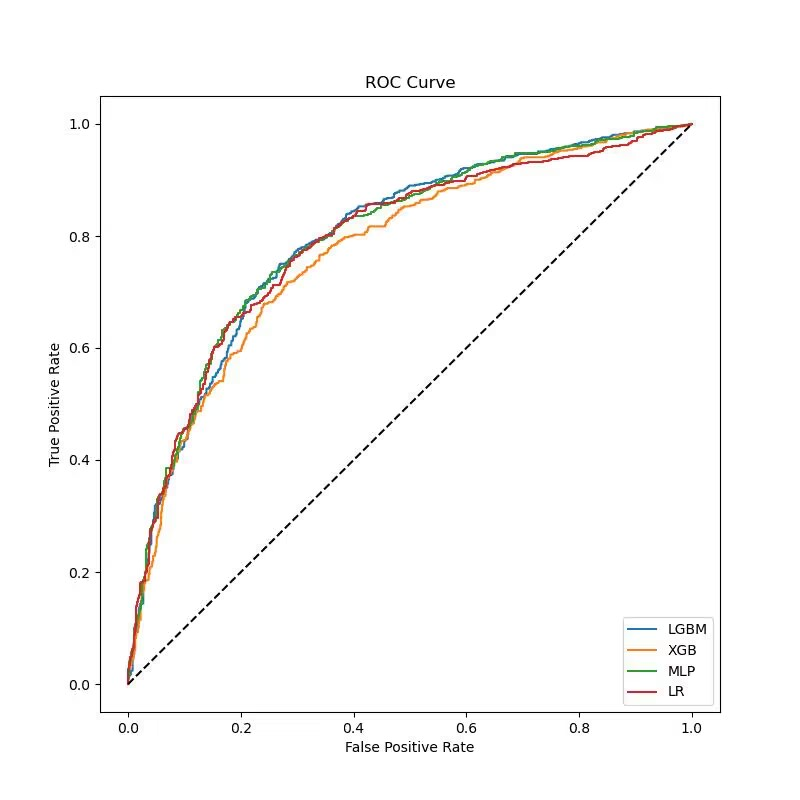
\includegraphics[width=12cm]{figures/ROC.jpg}
\caption{ROC curve} \label{fig:aa}
\end{figure}

We have further classified these 13 factors into five categories: situation, morale, physical strength, technical level, and whether they are the serving party. (to write) Starting from the category, if two variables within the same category have strong positive covariance, they are considered to have a high correlation and are merged through linear weighting. Through this method, we ultimately reduced the variables to eight. (to write) We use $y_i,1\leq i\leq8$ to represent these final 8 variables. We conducted a binary logistic regression analysis on these 8 variables again, and the analysis results are shown in Table 5. 

Among them, $y_1$ is related to the set/name/point that the player has already won, $y_2$ is related to whether they serve for themselves, $y_3$ is related to whether the player hits an unobstructed winning serve, $y_4$ is related to whether the player hits an unobstructed winning shot, $y_5$ is related to whether there is an forced error, $y_6$ is related to the distance the player runs in the game, $y_7$ is related to the score the player wins in the front court, the number of times they go to the front court, the number of successful breaks, and the speed of serving, $y_8$ is related to whether to serve and the speed of serving.
% Please add the following required packages to your document preamble:
% \usepackage{booktabs}
% \usepackage{longtable}
\begin{longtable}[c]{cccccc}
	\toprule
	\textbf{Sign}  & \textbf{B}       & \textbf{Standard Deviation} & \textbf{Wald}   & \textbf{Significance} & \textbf{Exp(B)}     \\* \midrule
	\endfirsthead
	\endhead
	$y_1$ & -1.688  & 0.234              & 51.969 & 0.235        & 0.185      \\* \midrule
	$y_2$ & -10.001 & 2.199              & 20.695 & 0.317        & 0.000      \\* \midrule
	$y_3$ & 0.216   & 0.198              & 1.195  & 0.274        & 1.242      \\* \midrule
	$y_4$ & 0.779   & 0.211              & 13.655 & 0.183        & 2.180      \\* \midrule
	$y_5$ & -1.155  & 0.169              & 46.943 & 0.221        & 0.315      \\* \midrule
	$y_6$ & 0.199   & 0.165              & 1.455  & 0.228        & 1.220      \\* \midrule
	$y_7$ & 3.733   & 0.474              & 62.125 & 0.302        & 41.800     \\* \midrule
	$y_8$ & 13.689  & 2.367              & 33.457 & 0.231        & 881141.288 \\* \bottomrule
	\caption{Binary Logistic Regression Analysis}
	\label{tab:my-table}
\end{longtable}



\subsection{Model Building}
\subsubsection{Model Selection}
In this task, we use machine learning models to learn game data based on the 8 features selected above, in order to predict real-time scores. We selecte a total of 5 machine learning models: LGBM, XGB, SVC, MLP and LR. We define samples with scores as positive samples and samples without scores as negative samples. 

\subsubsection{Evaluation Metrics}

We chose Accuracy, Precision, and AUC as the evaluation metrics for the model. The last two metrics can to some extent reflect the predictive ability of the model for positive samples. 

\subsubsection{Results Analysis}

We use these five models to learn match data and predict real-time scores during the competition process. The final performance results of the models are shown in Table 6. The ROC curve drawn is shown in Figure 7. It can be seen that the MLP model has shown advantages in both Acc, Prec, and AUC.

% Please add the following required packages to your document preamble:
% \usepackage{booktabs}
% \usepackage{longtable}
\begin{longtable}[c]{llll}
	\toprule
	\textbf{Model} & \textbf{Acc}.  & \textbf{Prec}. & \textbf{AUC}   \\* \midrule
	\endfirsthead
	\endhead
	LGBM  & 0.731 & 0.745 & 0.732 \\* \midrule
	XGB   & 0.713 & 0.697 & 0.714 \\* \midrule
	SVC   & 0.733 & 0.740 & 0.733 \\* \midrule
	MLP   & 0.738 & 0.754 & 0.738 \\* \midrule
	LR    & 0.728 & 0.737 & 0.728 \\* \bottomrule
	\caption{Results of the Models}
	\label{tab:my-table}
\end{longtable}

The MLP model, also known as the Multilayer Perceptron, is a feedforward artificial neural network model mainly used for classification and regression problems in machine learning and deep learning. MLP consists of an input layer, one or more hidden layers, and an output layer. Each neuron is connected to each neuron in the next layer and the input is transformed using an activation function. During the training process, MLP minimizes the loss function through backpropagation algorithm to achieve classification or regression goals.

In this task, due to the high dimensionality of the data, the advantage of MLP in processing high-dimensional data is reflected. At the same time, the large number of neurons and layers in MLP have strong expressive abilities, which can better learn complex patterns and structures in data.

We visualize the prediction results of the MLP model and plot the actual real-time scores and predicted actual scores of two players in a game, as shown in Figure 8.

\begin{figure}[h]
\centering
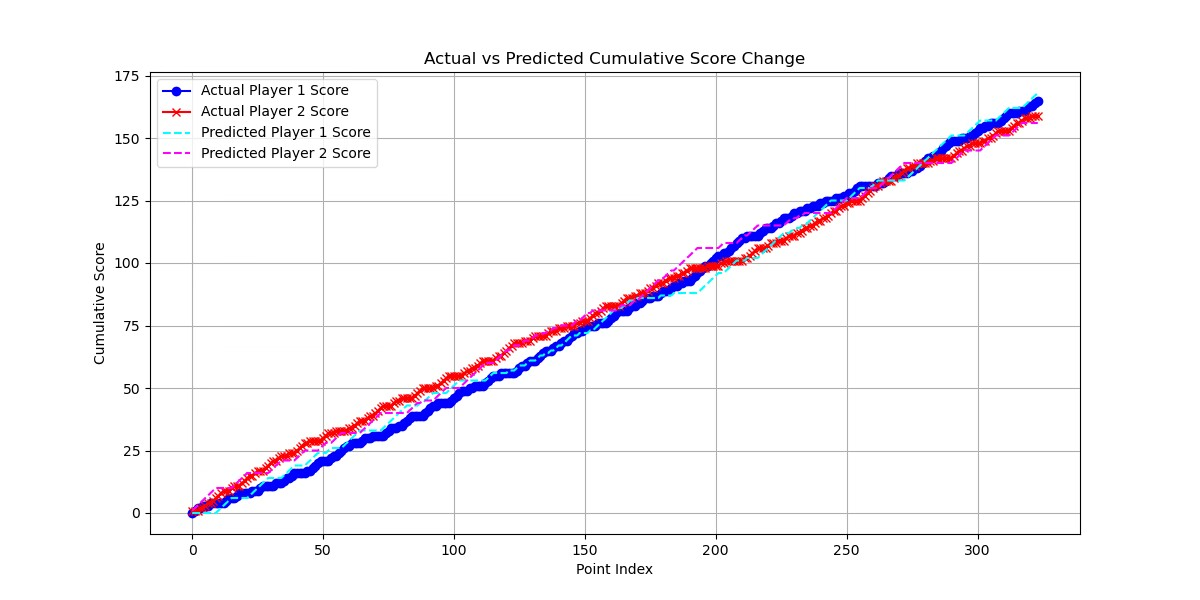
\includegraphics[width=12cm]{figures/replace.JPG}
\caption{Rusults of MLP} \label{fig:aa}
\end{figure}


\section{Changes in the Trend of Tennis Matches}
\subsection{Overall}
Firstly, we will define "changes in competition trends". Then we will use clustering methods according to the definition to find a turning point in a match. Finally, we will redesign the model and predict the turning points in the match based on the 8 variables in section 4.2.

\subsection{Data Processing}
In this task, we reused the MLP model to predict the final scores of each game in each match, and ultimately obtained the scores of two players in different games in each match.

\subsection{Task Definition}
After obtaining the scores of two players in different games of the same match, we subtract the scores of these two players to obtain the difference in their scores. We can think of it this way: in two consecutive games, if the difference in scores between the first and second players in the first game is positive, and the difference in scores between these two players in the second game is negative, then it is considered that during this match period, the competition is developing in a direction that is favorable to the second player. 

In this issue, we need to focus on the changes in the difference in game scores between two players over a continuous period of time. The difference in scores scored by players in consecutive games can to some extent reflect the changes in the trend of the match. To study the difference in scores between two players, we need to subtract the difference in scores between adjacent games. Through the following formulas, we can have a more intuitive understanding:
\[
	\bigtriangleup P_i = S_{1i} - S_{2i}
\]
\[
	\bigtriangleup TP_i = \bigtriangleup P_{j + 1} - \bigtriangleup P_j
\]
Among them, $S_{1i}$ represents the score of the first player in the i-th game, and $S_{2i}$ represents the score of the second player in the i-th game. $P_i$ represents the difference in scores between the two players in the i-th game. $TP_i$ represents the difference in scores between the j+1-th game and the j-th game. In this task, we aim to identify the turning points in the competition process by studying the changes in $TP_i$.

Meanwhile, we also continue to observe the turning points in a match from the point dimension. Similarly to the above definition, we study the difference in the probability of two players scoring in each score, and then we will perform a difference operation on the probability of two players scoring in steps of 2, which we consider to be a moderate scale. The formulas are as follows:
\[
	\bigtriangleup prob_i = p_{1i} - p_{2i}
\]
\[
	\bigtriangleup dp_i = \bigtriangleup prob_{j + 2} - \bigtriangleup prob_j
\]
Among them, $p_{1i}$ represents the probability of the first player getting the i-th point, and $p_{2i}$ represents the probability of the second player getting the i-th point. $prob_i$ represents the difference in the probability of two players scoring on the i-th point. $dp_i$ represents the difference in probability between the jth+2nd score and the jth score.

\subsection{Prediction of Turning Points}
\subsubsection{KMeans Clustering}
K-means is a typical clustering analysis method that aims to group similar data points together to form K clusters. In this method, a cluster is composed of data points, and the data points within the cluster are similar to each other, while the data points in different clusters are not similar to each other.

The basic process of KMeans is as follows:
\begin{enumerate}
  \item Specify the number of clusters to form, denoted as K.
  \item Randomly select K data points from the dataset as the initial cluster centers.
  \item For each data point in the dataset, calculate its distance from each cluster center and assign it to the cluster represented by the nearest cluster center.
  \item Update the average data points for each cluster as the new cluster center.
  \item Repeat steps 3 and 4 until the stop condition is met. The stopping condition can be that the change in cluster center is less than a certain threshold, the preset number of iterations is reached, or the cluster allocation of data points no longer changes.
  \item In the end, K clusters were obtained, and each data point was assigned to a cluster.
\end{enumerate}

\subsubsection{Task Processing}
In this task, we perform KMeans clustering on $PT_i$ in section 6.3 to capture a turning point in a match. We mainly select the final with the match id 17015 as the research object to conduct cluster analysis on the turning points of this competition. The clustering graph we obtained is shown in Figure 10. These points are vertically divided into five clusters, and the red and blue dots marked in the graph represent the largest 20\% of these points and the smallest 20\% of these points. These red and blue dots are points with significant differences between consecutive games, and we believe these points are turning points during the game. Meanwhile, we also perform the same work on $dp_i$ in section 6.3, and the results are shown in Figure 11. 

\begin{figure}[h]
\centering
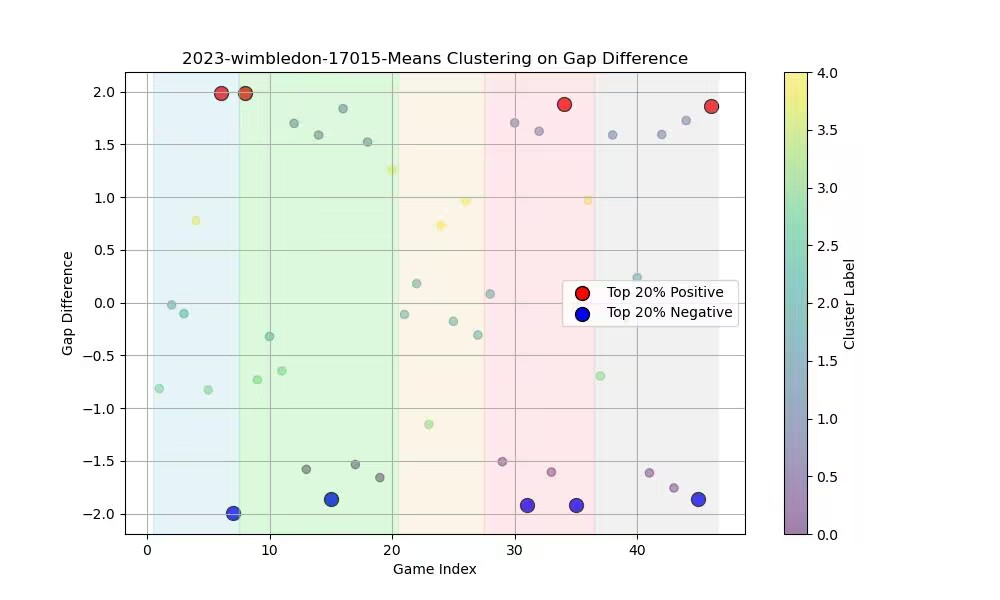
\includegraphics[width=12cm]{figures/KMeans.jpg}
\caption{KMeans Results in Games} \label{fig:aa}
\end{figure}

\begin{figure}[h]
\centering
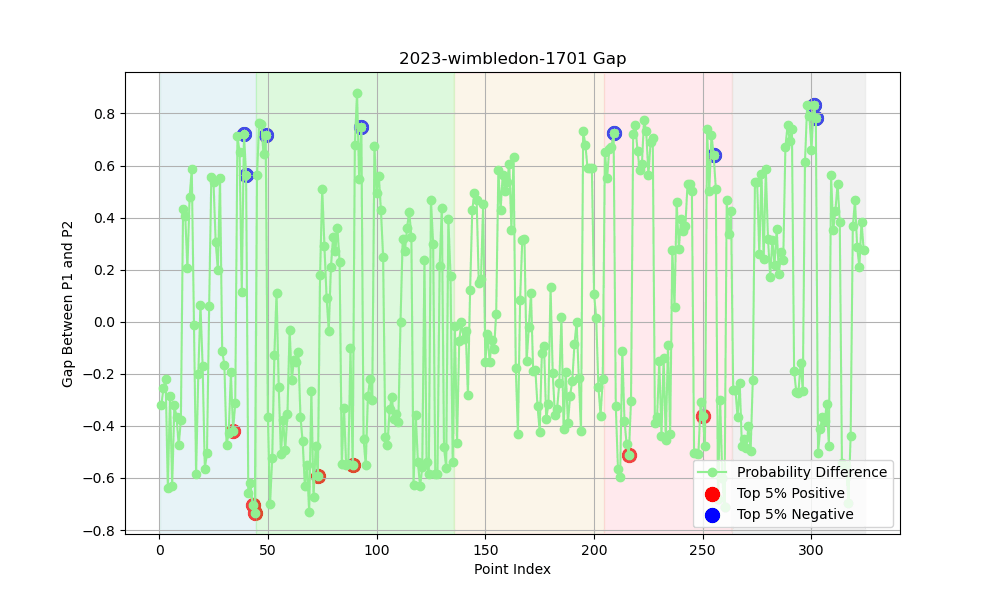
\includegraphics[width=12cm]{figures/Kmeans2.png}
\caption{KMeans Results in Points} \label{fig:aa}
\end{figure}

\subsubsection{Data Annotations}
At this step, we found that there are a few data points obtained through the game dimension, which is not conducive to our further processing. Therefore, in the subsequent process, we still choose to perform the task on the point dimension.

Next, we will annotate the points in Figure 11. We believe that the red dots appearing in Figure 11 represent the direction of the match in favor of the first player, and we label these dots as "1"; The blue dots appearing in Figure 11 represent the development of the competition in favor of the second player, and we label these dots as "-1"; For the other points that appear in the graph, we believe they will not have an impact on the competition trend and label them as "0". Next, we will redesign the model to predict the turning points of the competition based on the 8 variables mentioned in Section 5.2, which are labeled as "1", "0", and "-1".

\subsubsection{SVC Support Vector Machine}
Read the just annotated data, use $y_1$ to $y_8$ as features, and use inflection points as labels. Next, divide the training set and test set, randomly select a match (such as' 2023-wimbledon-1701 ') as the test set, and divide the remaining matches into the training set. Use SVC for training and verify on the test set. At the beginning, our results were not ideal. We noticed that the proportion of data labeled as "0" in the dataset was very large, with only a few labeled as "1" or "-1", which is consistent with the situation where only a few scores are turning points in the game. Therefore, we use the class\_weight of SVC. The weight parameter is set to 'balanced', which focuses more on minority categories and gives greater weight in inverse proportion to the number of samples. Meanwhile, we also use SMOTE for oversampling to better address class imbalance. However, sometimes overfitting may occur, and we address this issue by adding noise by incorporating random perturbations into the data. In the end, our prediction accuracy for turning points reached 83.33\%, which is relatively ideal.

\subsubsection{Weight Analysis}
We assess the weights of the 8 variables in SVC to explore which factors have the greatest impact on the turning point. The weight pie chart of 8 variables is shown in Figure 12. We find that $y_6$, $y_1$, and $y_7$ are the most important factors affecting the turning point. According to the meaning of the symbol y in Section 5.2, we know that running distance, the score won in the front court, the number of times to go to the front court, successful breaking, serving speed, and the set/name/point already won are important factors that affect the turning point of the game.

\begin{figure}[h]
\centering
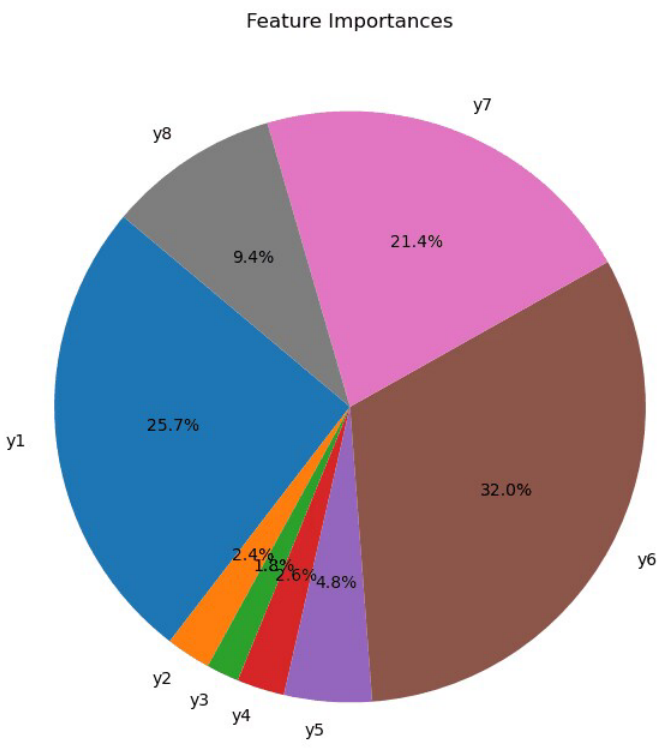
\includegraphics[width=12cm]{figures/Snipaste_2024-02-06_04-27-43.png}
\caption{Weight Pie Chart of 8 Variables} \label{fig:aa}
\end{figure}


\subsection{Advice for the Player}
Based on the previous analysis, for tennis players, we provide the following suggestions:
\begin{enumerate}
  \item Based on the opponent's playing style, determine whether they are inclined to hold the ball or quickly net. If the opponent frequently goes online quickly, it is recommended to increase the frequency and efficiency of the internet to reduce running distance.
  \item Analyze the scoring situation of oneself and opponents in the front court. If the opponent scores high in the front court, it is recommended to strengthen the serving and receiving techniques, improve the success rate of the net, or increase the stability of the baseline confrontation.
  \item Adjust the frequency of going to the front court according to the opponent's playing style. If the opponent likes to play deep balls, they can use more angles and depth to guide them to the front of the net.
  \item Improving the success rate of breaking is the key to winning the game. Understand the opponent's serving habits, such as which serving routes the opponent is weaker on, and increase attack intensity in these positions.
  \item Using the advantage of serving, if the ball is fast, you can try serving and surfing tactics; If the ball speed is not particularly fast, you can focus on the accuracy and rotation of the serve to create difficulties for the opponent's reception.
  \item Always maintain a positive attitude. If leading in a certain stage, continue to maintain; If you are at a disadvantage in a certain aspect, you need to adjust your mentality in the upcoming matches.
\end{enumerate}


\section{Verification of Model Generalization Ability}
In order to verify the generalization ability of the model, we chose a French Open final by Djokovic in 2016 as additional data. Our predicted turning point graph is shown in Figure 13.

For the 2016-frenchopen-1701 game, Djokovic (player1) performed well at the beginning and scored continuously. In the second game, Djokovic's form declined significantly, and Murray (player2) easily won. Next, Djokovic's performance rebounded slightly, but the predicted value was still less than 0. At the end of the fifth inning, the first turning point was reached, and Djokovic's performance significantly improved, but he still suffered losses. Murray won four consecutive games. In the sixth inning, both sides scored alternately, and Djokovic won the game with a slight advantage. In the seventh game, both sides continued to score alternately. Although Djokovic lost the game, he reached a turning point towards the end, his form improved significantly, and he successfully won the eighth game. Next, Djokovic's form declined again, and Murray seized the opportunity to score continuously. Although Djokovic recovered and his performance improved significantly, he was unable to recover. In the end, Murray achieved his first set victory.

In the second set, Djokovic's performance fluctuated slightly, but overall improved, with predicted values mostly above zero. In the end, he successfully won the set 6-1.

At the beginning, Djokovic's performance in the third set was average, but his form continued to improve and he won five consecutive games. Although his performance in the seventh game was slightly poor, he improved in the eighth game and ultimately won the set.

Djokovic entered the final set with a large score of 2:1, and both sides had a winner or loser. In the end, Djokovic won. This is basically consistent with our predicted turning point graph.

In the prediction of another Australian Open women's singles match, the model's results were not ideal, and we speculate that there may be objective factors such as venue and weather. At the same time, gender differences and age factors can have other impacts such as insufficient physical strength, making our model predictions not very accurate.

However, we did not make too many assumptions about the model and did not limit it to specific types of events, venues, or the sport of tennis. Therefore, our model can adapt to most game data and has good generalization ability.



\begin{figure}[h]
\centering
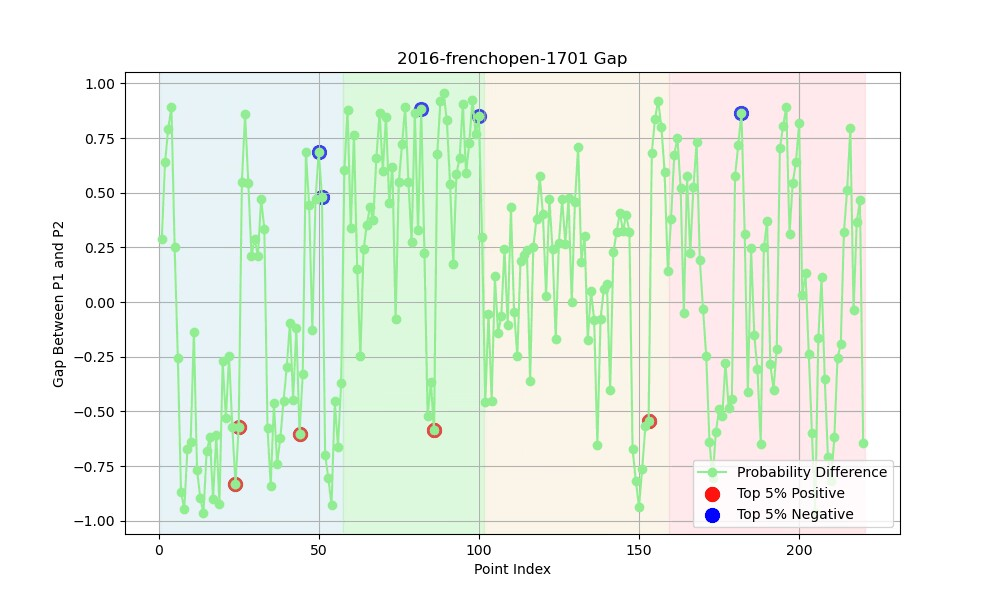
\includegraphics[width=12cm]{figures/D2016.png}
\caption{Turing Points in 2016 Match} \label{fig:aa}
\end{figure}




\section{Strengths and Weaknesses}
\subsection{Strengths}
\begin{itemize}
  \item Due to the use of kernel functions to map input data to high-dimensional feature spaces, the SVC model makes the originally nonlinear data linearly separable in a new space, thus possessing good generalization ability. We also verified this in Section 7
  \item The model has high accuracy. Due to our attention to detail in feature processing, the 8 features we selected have strong correlation. Therefore, the SVC model can better learn the spatial data distribution during the learning process, thereby improving the accuracy of the model.
  \item Due to the introduction of noise during the parameter adjustment process, we controlled the class\_ The weight parameter is used to avoid model bias caused by sample bias, making the model highly robust.
\end{itemize}

\subsection{Weaknesses}
\begin{itemize}
    \item The model focuses too much on real-time scoring from a micro perspective. In fact, scoring or losing one or two points at the beginning of a game does not have a significant impact on the mid to late stages of the game.
\end{itemize}

\section{Letter to the Coach}

\begin{letter}{Dear Coach:}

\end{letter}
Thank you very much for your inquiry! We have conducted a detailed study on momentum in tennis matches based on the match data you provided. We will introduce the role of momentum in tennis matches based on our research and provide some guidance to players.

Firstly, regarding the concept of momentum, we believe that momentum is an indicator that reflects the changes in the trend of a game, and it is influenced by a large number of different factors between the players on both sides. At the beginning, we proposed a performance model to measure momentum. The performance model considers the impact of serving and morale on performance. In terms of serving, we have considered two factors: serving score and breaking, and in terms of morale, we have considered the factor of consecutive scoring. In fact, as you might think, when a player scores a serve or completes a break, their performance must be fantastic. Meanwhile, when he starts scoring continuously, it also indicates that his form is in a very hot state. We measure a contestant's performance based on these points and give them the performance points they should receive at each moment. After a match, the player with a higher performance score should have won the game. If not, it indicates that our model incorrectly predicted the player's performance. It is gratifying that we validated our model in 31 matches, with only 3 predictions failing and an accuracy rate of 90.323\%. Moreover, we also characterize the performance into curves and observe the real-time changes of the curves, which are basically consistent with the actual victory or defeat situation of the set. It can be said that our model has shown advantages in predicting the performance of athletes. We believe that the performance score predicted by our performance model can roughly reflect the momentum in the game.

However, at first you were skeptical about the effect of momentum, right? You used to think that the fluctuations in the game and the consecutive scores of players were random events, right? After our research, we have verified that momentum actually plays a role in competitions, and the consecutive scores of players are not random events. We conducted a chi square test on the output results of the performance model and the actual outcome of the match, with a chi square statistic of 15.81. At the same time, we also tested the Pearson correlation coefficient of the performance model's real-time prediction results and real-time score situation for each score, and calculated the Pearson correlation coefficient to be 0.366. Because our performance model can roughly reflect the momentum during the competition, we believe that momentum is not ineffective during the competition. In addition, we also tested the distribution of consecutive scores of players. If it is really a random event, the distribution of consecutive scores should be a normal distribution or geometric distribution, but in reality, neither is true. So, consecutive scoring in a game is not a random event.   

We continued to delve deeper and selected 16 factors that may affect the score. After screening through binary logistic regression and covariance matrix, we ultimately identified 8 factors that are related to the score, which we believe are the factors that affect momentum. Next, we will continue to study the turning points in the competition - which is also the most direct manifestation of momentum. We first defined the turning points in a game, and then used KMeans clustering to cluster the potential turning points in the game data, ultimately obtaining the predicted turning points. We designed a support vector machine model to learn turning points based on the 8 factors mentioned earlier, in order to predict turning points in competitions. After a series of adjustments to the model, our prediction accuracy ultimately reached 83.33\%. Then, we continue to use support vector machine models to analyze the importance level of these 8 factors. The final result indicates that the importance of factors such as running distance, score earned in the front court, number of trips to the front court, successful breaking, serving speed, and score already won is relatively high. Therefore, when guiding your competitors to participate in competitions, you can give them the following suggestions to deal with fluctuations in the competition:
\begin{itemize}
  \item Before the game, it is necessary to analyze the opponent's playing style and determine whether they tend to hold the ball or quickly score. If the opponent frequently goes online quickly, it is recommended to increase the frequency and efficiency of the internet to reduce running distance.
  \item To understand the opponent's serving habits and improve the success rate of breaking serve.
  \item Always maintain a positive attitude. If leading in a certain stage, continue to maintain; If you are at a disadvantage in a certain aspect, you need to adjust your mentality in the upcoming matches.
\end{itemize}

We greatly appreciate your trust in our team and hope that our work and analysis can be helpful to you.

\begin{letter}{}

Best,

\end{letter}
MCM Team \#2412631



\begin{thebibliography}{99}
\bibitem{1} T. Barnett and S. R. Clarke, "Combining player statistics to predict outcomes of tennis matches," in IMA Journal of Management Mathematics, vol. 16, no. 2, pp. 113-120, Jan. 2005, doi: 10.1093/imaman/dpi001.
keywords: {tennis;Australian Open;scoring systems;Excel;gamblinga},
\bibitem{2} Dietl, Helmut \& Nesseler, Cornel. (2017). Momentum in tennis: Controlling the match. International Journal of Sport Psychology. 48. 10.7352/IJSP2017.48.459. ,
Addison-Wesley Publishing Company, 1986.
\bibitem{3}\url{https://theanalyst.com/eu/2022/03/capturing-momentum-in-tennis/}
\end{thebibliography}

\AImatter

\begin{ReportAiUse}{9}
\bibitem{AI1}
GPT-4\\
Query1: Please help me search the articles about factors affecting the tennis game\\
Output: I have found some articles analyzing the factors that affect the changes in the situation in tennis matches, which explore this issue from different perspectives.

An article from ResearchGate discusses the role of momentum in tennis matches, particularly exploring the impact of winning the last set on the probability of winning the final match. This article also analyzes the impact of game points on momentum, as well as whether game rounds have an impact on momentum. Research has found that winning the second to last set with a significant advantage can significantly increase the chance of winning the last set, while winning the second to last set with a small advantage is likely to result in losing the last set and the entire game, which is called anti momentum.

Another article from The Analyst provides a detailed explanation of how leverage and momentum are calculated in tennis matches and how they affect match results. Leverage is used to measure the importance of a single score to the final outcome of a game, that is, how the probability of a player winning the game changes with the outcome of the next point. Momentum aims to describe which player in the game is in a state of control, that is, who is winning more points and important (high leverage) points. By modeling the data of 1.5 million points on the WTA Tour from 2012 to 2020, researchers were able to predict the impact of each point on the game results and calculate momentum based on this to quantify the dominant moments in the game.

These studies provide in-depth analysis and a comprehensive understanding of the changing factors in tennis matches. If you are interested in detailed information, you can refer to these articles for more insights..

There are many other sorting algorithms available such as bubble sort, insertion sort, merge sort, quick sort, heap sort, and more. Each of these algorithms has its own advantages and disadvantages. You can learn more about them on GeeksforGeeks and Programiz.

I hope this helps!

\bibitem{AI2}
Query2: can you tell me more about chi square test?\\
Output: The Chi-square test is a statistical method used to determine if there is a significant difference between observed frequencies and the frequencies expected under a specific hypothesis. It's commonly used in research to test relationships between categorical variables. For example, it can help determine if the distribution of some characteristic differs across groups. The test calculates a Chi-square statistic, which compares the observed values with the values expected according to the null hypothesis (no association between variables). If the calculated statistic is higher than the critical value from Chi-square distribution tables, the null hypothesis is rejected, indicating a significant difference or association.


\bibitem{AI3}
Query3: how to set a list in latex\\
Output: In LaTeX, lists can be created using the itemize environment for unordered lists or the enumerate environment for ordered lists. Here's how to set them up:

Unordered list (using itemize):
\begin{lstlisting}[language=tex]
\begin{itemize}
  \item First item
  \item Second item
  \item Third item
\end{itemize}
\end{lstlisting}
Ordered list (using enumerate):
\begin{lstlisting}[language=tex]
\begin{enumerate}
  \item First item
  \item Second item
  \item Third item
\end{enumerate}
\end{lstlisting}
These environments automatically handle item markers (bullets or numbers) and spacing between items. You can nest these environments to create multi-level lists.

\end{ReportAiUse}

\end{document}
%% 
%% This work consists of these files mcmthesis.dtx,
%%                                   figures/ and
%%                                   code/,
%% and the derived files             mcmthesis.cls,
%%                                   mcmthesis-demo.tex,
%%                                   README,
%%                                   LICENSE,
%%                                   mcmthesis.pdf and
%%                                   mcmthesis-demo.pdf.
%%
%% End of file `mcmthesis-demo.tex'.
